\documentclass{SeminarV2}
\usepackage{graphicx}
\usepackage[utf8]{inputenc}
\usepackage{amssymb,amsmath,array}

%***********************************************************************
% !!!! IMPORTANT NOTICE ON TEXT MARGINS !!!!!
%***********************************************************************
%
% Please avoid using DVI2PDF or PS2PDF converters: some undesired
% shifting/scaling may occur when using these programs
% It is strongly recommended to use the DVIPS converters.
%
% Check that you have set the paper size to A4 (and NOT to letter) in your
% dvi2ps converter, in Adobe Acrobat if you use it, and in any printer driver
% that you could use.  You also have to disable the 'scale to fit paper' option
% of your printer driver.
%
% In any case, please check carefully that the final size of the top and
% bottom margins is 5.2 cm and of the left and right margins is 4.4 cm.
% It is your responsibility to verify this important requirement.  
% If these margin requirements and not fulfilled at the end of your file generation process, please use the following commands to correct them.  Otherwise, please do not modify these commands.
%
\voffset 0 cm \hoffset 0 cm \addtolength{\textwidth}{0cm}
\addtolength{\textheight}{0cm}\addtolength{\leftmargin}{0cm}

%***********************************************************************
% !!!! USE OF THE SeminarV2 LaTeX STYLE FILE !!!!!
%***********************************************************************
%
% Some commands are inserted in the following .tex example file.  Therefore to
% set up your Seminar submission, please use this file and modify it to insert
% your text, rather than staring from a blank .tex file.  In this way, you will
% have the commands inserted in the right place.

% Edited by Martin Bogdan.

\begin{document}
%style file for Seminar manuscripts
\title{Simulation der Histonmodifikation}

%***********************************************************************
% AUTHORS INFORMATION AREA
%***********************************************************************
\author{Max Hild
% DO NOT MODIFY THE FOLLOWING '\vspace' ARGUMENT
\vspace{.3cm}\\
%
% Addresses and institutions (remove "1- " in case of a single institution)
\emph{Abgegeben bei: Dr. J\"{o}rg Galle, Prof. Dr. Markus Scholz}
% Remove the next three lines in case of a single institution
\vspace{.1cm}\\
Universit\"{a}t Leipzig, Institut f\"{u}r medizinische Informatik, Statistik und Epidemiologie\\
Neues Augusteum, Augustuspl. 10, 04109 Leipzig - Germany
}


%***********************************************************************
% END OF AUTHORS INFORMATION AREA
%***********************************************************************

\maketitle

\begin{abstract}
  \sloppy
  GWAS (Genome-Wide Association Studies) erklären nur einen kleinen Teil der Heritabilität von 
  genetischen Varianten, die mit komplexen Erkrankungen assoziiert sein k\"{o}nnten.
  \cite{mcclellan-2010} Ein großer Teil der Heritabilität wird heutzutage epigenetischen Prozessen
  zugeschrieben.
    
  Dazu gehört in Eukaryoten vor allem die reversible chemische Modifikation der Histonproteine. \cite{prohaska-2010}
  Diese Mechanismen sind dynamisch und k\"{o}nnen durch Umweltfaktoren beeinflusst werden, 
  was sie zu einem spannenden Forschungsfeld macht. Die vorliegende Simulation soll die 
  Histonmodifikation basierend auf dem komputationalen Modell von Prohaska et al. simulieren.
  Dabei wurde der deterministische, regelbasierte Ansatz aus der Publikation mit einer 
  stochastischen Markovsimulation verglichen und letztendlich kombiniert.
  \end{abstract}
  
\section{Einleitung}
Die Heritabilit\"{a}t von Ph\"{a}notypen besser zu erforschen l\"{a}sst Forscherinnen und Forscher leichter
nachvollziehen, wie die genetische Information kodiert ist.
Prohaska et al. argumentieren, dass die Bedeutung des regulatorischen Systems der Epigenetik f\"{u}r die Vererbung gro{\ss} ist.
Sie skizzieren ein komputationales Modell, das Reader und Writer Proteine verwendet, die durch eine zugrundeliegende Regulationsfunktion die DNA Replikation sowie Transkription steuern.
Dieses System wird in Prohaska et al. mit einem deterministischen System beschrieben, das die Dynamik der epigenetischen Zust\"{a}nde an Histonen in einem Genom simuliert.
Das regulatorische System der Epigenetik wird als ein Schlüssel zur Erklärung der fehlenden Heritabilität gesehen.
Diese anerkannte Theorie wird durch Evidenz unterstützt. Jedoch ist es noch ein Forschungsgegenstand, wie genau die komplexeren Systeme, die bei Eukaryoten zu finden sind, gesteuert werden. \cite{prohaska-2010}
Auch aus der Sicht von Bannister {\&} Kouzarides spielen Histonmodifikationen eine zentrale Rolle im epigenetischen Code. 
Sie beschreiben die verschiedenen Writer, Eraser und Reader von Histonmarken und deren Einfluss auf Transkription, DNA-Reparatur und Chromosomenkondensation \cite{bannister-2011}.  
Transgenerationale Epigenetikstudien zeigen zudem, dass bestimmte epigenetische Markierungen selbst \"{u}ber mehrere Generationen hinweg erhalten bleiben k\"{o}nnen und so zur fehlenden Heritabilit\"{a}t beitragen \cite{tollefsbol-2014}.
Diese Forschung deckt sich mit der Empfehlung von McClellan et al.
die in ihrer Arbeit ein Pl\"{a}doyer f\"{u}r die Forschung
nach der fehlenden Heritabilit\"{a}t halten. 

\begin{quote}
  \sloppy
  Eine der gr\"{o}{\ss}en Hoffnungen an die GWAS war, dass man - 
  genauso wie eine Vielzahl von mendelschen Erkrankungen auf DNA-Ebene 
  eingegrenzt und das beteiligte Gen samt den Mutationen identifiziert werden konnte - 
  einfach von Einzelgen-Erkrankungen auf komplexe multigenetische Erkrankungen schlie{\ss}en k\"{o}nnte. 
  Das ist jedoch nicht eingetreten. Bef\"{u}rworter werden argumentieren, dass es funktioniert hat 
  und dass allerlei faszinierende Gene identifiziert wurden, die beispielsweise eine Pr\"{a}disposition 
  zu oder einen Schutz vor Diabetes oder Brustkrebs verleihen, aber die Tatsache bleibt, dass der Gro{\ss}teil 
  der Erblichkeit in diesen Erkrankungen nicht den durch GWAS identifizierten Loci zugeschrieben werden 
  kann, was eindeutig zeigt, dass dies nicht die universelle L\"{o}sung sein wird.
  \cite{mcclellan-2010}
\end{quote}

\section{Methoden}
Zentraler Bestandteil dieser Arbeit ist der Vergleich eines stochastischen Modells, welches auf Basis von Markov Ketten mittels \"{U}bergangswahrscheinlichkeiten die Histonmodifikation simuliert, mit einem Modell welches auf der Forschung von
Prohaska et al. basiert.
Sie beschreiben Chromatin als hierarchisches Informationssystem, in dem Reader- und Writerproteine chemische Markierungen auf Histonen setzen und auslesen. 
Diese Markierungen modulieren die Zugänglichkeit der DNA für Transkriptions- und Reparaturmaschinen.
Das Modell beschreibt die Histonmodifikation als ein deterministisches System.
Es definiert jeden Nukleosom‑Knoten durch zwei Flags für Acetylation (H3K27ac) und Methylation (H3K9me3) sowie einen Aktivitätsindikator. In jedem Zeitschritt werden alle Nukleosomen gleichzeitig nach folgenden Regeln aktualisiert: 
Ein Nukleosom erwirbt Acetylation, falls sein linker Nachbar bereits acetylierte Kennzeichnungen besitzt, andernfalls erhält es Methylation, falls sein rechter Nachbar methy­liert ist. Diese strikt logischen Booleschen Operationen werden in der Methode \texttt{applyDeterministicProhaskaRules()} umgesetzt.
Diese Zustände entscheiden nach heutiger Ansicht darüber, ob und wie die DNA an dieser Stelle für die Transkription verwendet werden kann.
Die simplere Ansicht, dass die Zustände des Chromatins binär seien, wurde widerlegt. Filon et al. erkannten durch Principal Component Analysis fünf verschiedene 
Typen von Chromatin. \cite{filon-2010}

\section{Prohaska-Modell, (deterministischer Ansatz)}
Das auf Prohaska et al. basierende Modell zeigt einen Ansatz, bei dem durch das Festlegen
von Regeln eine Vorhersage über die zukünftige Konstellation der Histonmodifikationen getroffen wird.
Dieser regelbasierte Ansatz hat den Vorteil, dass hierdurch Erkenntnisse aus der realen Welt in das Modell einfließen können.
Die Schwäche dieses Modells ist es jedoch, dass dadurch oft ein Endzustand erreicht wird, bei dem das Modell sich nicht mehr ändert.
Die verwendeten Regeln sind:
Acetylations-Writer (Aktivierungs-Regel):
Diese Regel modelliert, wie ein bereits acetylierter Nachbar (H3K27ac) ein Nukleosom “aktiviert” und selbst acetylieren lässt. Prohaska et al. sprechen hier von einem positiven Rückkopplungsschritt, der aktives Chromatin ausbreitet.
Methylations-Writer (Silencing-Regel):
Entspricht der Rekrutierung eines Methyltransferase-Komplexes (z. B. DNMT1), der einen Nukleosom re-methyliert und dadurch “stummschaltet”. Dies ist in ihrem Framework der Repressive Feedbackschritt, der in Konfliktsituationen immer Vorrang vor Acetylation hat.
Zudem wurde zufallsbasiert ein Eraser in das Modell aufgenommen der mit einer wählbahren Wahrscheinlichkeit einzelne Modifikationen löscht.
Da das Modell relativ schnell in einen stabilen Zustand konvergierte, wurde es mit einem Markovmodell erweitert, das zusätzliche zufällige Übergangswahrscheinlichkeiten definiert. \ref{fig:P_1000}

\subsection{Markov-Modell (stochastischer Ansatz)}
Die \"{U}berg\"{a}nge zwischen diesen Zust\"{a}nden 
werden durch ein stochastisches Modell gesteuert, das die 
biologischen Prozesse der Modifikation und Demodifikation nachbildet. 
Die Implementierung verwendet einen Markov-Prozess, bei dem die 
\"{U}bergangswahrscheinlichkeiten von den aktuellen Zust\"{a}nden benachbarter Histonstellen abh\"{a}ngen.
Jeder Zeitschritt besteht darin, für jede Histonstelle den nächsten Zustand basierend auf den definierten Übergangswahrscheinlichkeiten zufällig zu wählen. \ref{fig:M_1000}

\subsection{Kombiniertes Modell}
Zusätzlich zur zufälligen Auswahl wird im Modell eine deterministische Komponente integriert, indem die Prohaska-Regeln vor jedem stochastischen Schritt angewendet werden. Dadurch entsteht ein hybrider Ansatz, der sowohl deterministische Nachbarschaftsregeln als auch stochastische Veränderungen abbildet und somit biologisch realistischer sein könnte.
\ref{fig:PM_1000}
In der Analyse der Größe der Cluster sowie der Autokorrelation wird deutlich, dass der Unmethylierte Zustand über die Zeit abnimmt, jedoch auch durch zufällige Ereignisse wieder ansteigen kann.
Das bietet interessante Möglichkeiten für die Analyse der Auswirkung von Risikofaktoren, die über weitere Übergangswahrscheinlichkeiten modelliert werden könnten.\ref{fig:PM_1000_A}\ref{fig:PM_1000_C}

\subsection{Modellierung}
Die Simulation wird in Zeitschritten von 1 Zeiteinheit durchgef\"{u}hrt, wobei die \"{U}bergangswahrscheinlichkeiten f\"{u}r jeden Zustand und jede Nachbarschaftskonfiguration 
vor der Simulation basierend auf aktuellem Kenntnisstand festgelegt wird.
Die Simulation wird f\"{u}r eine bestimmte Anzahl von Iterationen durchgef\"{u}hrt, um die zeitliche Entwicklung der Histonestellen zu beobachten.
Die Histone (Sites, Orte) wurden auf 10 gesetzt, während die chemischen Histonmodifikationen auf 5 gesetzt wurden (States, Zustände).
Die folgenden Zust\"{a}nde wurden definiert:
\begin{itemize}
  \item \textbf{U}nmodifiziert (U): Histon ist nicht modifiziert.
  \item \textbf{M}ethyliert (M): Histon ist methyliert.
  \item \textbf{P}hosphoryliert (P): Histon ist phosphoryliert.
  \item \textbf{A}cetylisiert (A): Histon ist acetylisiert.
  \item \textbf{U}biquitiliert (U): Histon ist ubiquitiliert.
\end{itemize}

\textbf{Technische Details:}
Die \texttt{EpigeneticSite}-Klasse speichert den aktuellen Zustand (\texttt{ModificationState}) als Enum und stellt Methoden zum Setzen und Abfragen des Zustands bereit.
Das \texttt{Conditional Model} verwaltet eine Liste von \texttt{HistoneSite}-Objekten und erm\"{o}glicht den Zugriff auf benachbarte Stellen, was f\"{u}r die konditionalen \"{U}berg\"{a}nge notwendig ist.
In der \texttt{Main}-Klasse wird die Simulationslogik implementiert. Sie verwendet einen Zufallszahlengenerator, um stochastische \"{U}berg\"{a}nge gem\"{a}\ss den spezifizierten Wahrscheinlichkeiten durchzuf\"{u}hren. Die \"{U}bergangswahrscheinlichkeiten sind in einer Matrix abgelegt, die f\"{u}r jeden Zustand und jede Nachbarschaftskonfiguration die jeweilige Wahrscheinlichkeit enth\"{a}lt.
Die Ergebnisse werden nach jedem Zeitschritt in eine CSV-Datei geschrieben. Diese Datei enth\"{a}lt den Zustand jeder Histonstelle zu jedem Zeitpunkt.
F\"{u}r die Visualisierung wird ein separates Python-Skript verwendet, das die CSV-Datei einliest und sowohl eine Heatmap als auch eine Zeitreihe der Zustandsverteilungen erzeugt.
Darüberhinaus kann die Autokorrelation sowie die Clusterverteilung visualisiert werden.

\section{Ergebnisse}
Die Simulation erm\"{o}glicht es, die zeitliche Entwicklung der epigenetischen Zust\"{a}nde 
\"{u}ber mehrere Generationen zu beobachten. Abbildung \ref{fig:PM_1000} zeigt die Visualisierung der ersten Version einer Simulation.
Die Visualisierung besteht aus zwei Teilen: Die Heatmap wurde verwendet, um den Zustand jeder einzelnen Histonstelle \"{u}ber die Zeit darzustellen.
Das Liniendiagramm zeigt die H\"{a}ufigkeit jedes Zustands \"{u}ber die Zeit.

\section{Anwendung des stochastischen Modells mit realistischen Daten}
Im n\"{a}chsten Schritt wurde eine Visualisierung mit \"{U}bergangswahrscheinlichkeiten aus reellen Daten durchgef\"{u}hrt. Die f\"{u}r diese Simulation gew\"{a}hlten \"{U}bergangswahrscheinlichkeiten basieren auf quantitativen Sch\"{a}tzungen aus der Literatur.  
Hier wurden die Ergebnisse von Fu et al. (2010) genutzt, die mittels eines Bayes'schen Modells an humanen FMR1-Daten folgende Raten ermittelt haben \cite{fu-2010}:
\begin{itemize}
  \item \textbf{Fehlerrate der Methylierungs-Erhaltung (Maintenance failure)}: 0{,}024 pro Zellteilung  
  \item \textbf{De-novo-Methylierungsrate (Elternstrang)}: Median 0{,}08 (80 \% CI: 0,04-0,13)  
  \item \textbf{De-novo-Methylierungsrate (Tochterstrang)}: Median 0{,}07 (80 \% CI: 0,04-0,11)  
\end{itemize}
Es wurde für die Wahrscheinlichkeit einer Methylierung der Wert des Tochterstrangs,
also 0,07, verwendet. Die Wahrscheinlichkeit der De-novo-Methylierung wurde auf 0,24 gesetzt. Die Ergebnisse der Simulation mit den \"{U}bergangswahrscheinlichkeiten nach Fu et al. (2010) sind in Abbildung \ref{fig:Fu_1000} dargestellt.
Die Ergebnisse zeigen deutliche Muster in der r\"{a}umlichen und zeitlichen 
Verteilung der epigenetischen Zust\"{a}nde. Insbesondere kann man beobachten, wie sich die Methylierungszust\"{a}nde in bestimmten Regionen zusammenh\"{a}ufen und wie sich die Modifikationen mit den gewählten Wahrscheinlichkeiten \"{u}ber die Zeit entwickeln.

\section{Diskussion}
Im Vergleich mit der deterministischen Implementierung von Prohaska et al. zeigt das stochastische Modell eine größere Variabilität in der zeitlichen Entwicklung der Histonzustände. Dies könnte darauf hindeuten, dass das stochastische Modell besser geeignet ist, um die biologischen Prozesse der Histonmodifikation und deren Einfluss auf die Genexpression zu erfassen. Die Ergebnisse der Simulationen zeigen, dass das stochastische Modell in der Lage ist, komplexe Muster zu erzeugen, die in der Natur beobachtet werden können.
Das deterministische Modell zeigt eine größere Stabilität, die sich in der Bildung stabiler Cluster widerspiegelt. Diese Stabilität könnte in biologischen Systemen von Bedeutung sein, da hier das Ziel eine robuste Regulation der Genexpression wäre.
Die Kombination des stochastischen und des deterministischen Modells weist als Erweiterung den realistischsten Verlauf auf, und nutzt die Vorteile beider Ansätze. 
Das kann als Äquivalent der biologisch gewollten Anpassung des regulatorischen Systems und der Einflüsse durch die Umwelt betrachtet werden.

\subsection{Weitere Nutzung}
Im Modul main.cpp kann das Modell vielfältig parametrisiert werden. Neben der Auswahl der verschiedenen Methoden (Markov sowie Prohaska-Regelbasiert) können auch aus der Forschung geschätzte Übergangswahrscheinlichkeiten sowie die Anzahl der Iterationen und die Anzahl der Histonstellen eingestellt werden.
Das ermöglicht eine vielfältige Nutzung des Modells um verschiedene Szenarien zu simulieren und deren Auswirkungen auf die Histonzustände zu analysieren.
Durch die Übergangswahrscheinlichkeiten könnten verschiedene Risikofaktoren, die das regulatorische System beeinflussen könnten, mit der regelbasierten Simulation kombiniert werden.

\subsection{Limitationen und Ausblick}
Obwohl das Modell viele Aspekte der epigenetischen Regulation abbildet, gibt es Einschr\"{a}nkungen:
\begin{itemize}
    \item Die \"{U}bergangswahrscheinlichkeiten sind aktuell statisch und basieren auf Literaturwerten oder Annahmen. Eine Kalibrierung mit experimentellen Daten sowie ein Training dieser k\"{o}nnte die Aussagekraft weiter erh\"{o}hen indem das epigenetische neuronale Netz erweitert wird.
    \item Die Validierung erfolgte bisher nur qualitativ. Eine quantitative Validierung gegen experimentelle Zeitreihen ist ein n\"{a}chster Schritt.
    \item Weitere epigenetische Mechanismen (z.B. Risikofaktoren, Messungen aus Studien Interaktion mit Transkriptionsfaktoren) k\"{o}nnten einfach integriert werden, um das Modell zu erweitern.
    \item Die Annahmen von Prohaska et al. müssten aktualisert und erweitert werden, um die Dynamik der Histonmodifikation bestmöglich abzubilden.
\end{itemize}

\section{Fazit}
Die C++ Implementierung der DNA-Histonmodifikation erm\"{o}glicht ein tieferes Verst\"{a}ndnis der dynamischen Prozesse, die der epigenetischen Regulation zugrunde liegen. Durch die Kombination von effizienter Simulation und anschaulicher Visualisierung k\"{o}nnen komplexe epigenetische Muster simuliert und analysiert werden.
Diese Art der Modellierung kann dazu beitragen, die fehlende Heritabilit\"{a}t besser zu verstehen, indem sie aufzeigt, wie epigenetische Mechanismen zur Vererbung ph\"{a}notypischer Merkmale beitragen k\"{o}nnen. 
Zuk\"{u}nftige Erweiterungen der Implementierung k\"{o}nnten eine parallele Simulation von Eltern und Kind Str\"{a}ngen beinhalten, um die transgenerationale Vererbung von epigenetischen Markierungen zu untersuchen.
Zudem könnte ein Messfehlerparameter eingeführt werden.
Die Nutzung von weiteren experimentellen Daten kann zur Validierung des Modells sowie zur Simulation spezifischer genetischer Erkrankungen genutzt werden, um potenzielle epigenetische Therapieans\"{a}tze zu identifizieren.
Weiterhin können mit dieser Implementierung Erwartungswerte basierend auf vergangenen Beobachtungen errechnet werden. So kann \"{u}ber l\"{a}ngere Zeit beobachtet werden, wie sich das epigenetische regulatorische System verhalten w\"{u}rde, wenn bestimmte Annahmen \"{u}ber die Histonmodifikation der Wahrheit entsprechen.

\section{Abbildungen}


\begin{figure}[htbp]
  \centering
  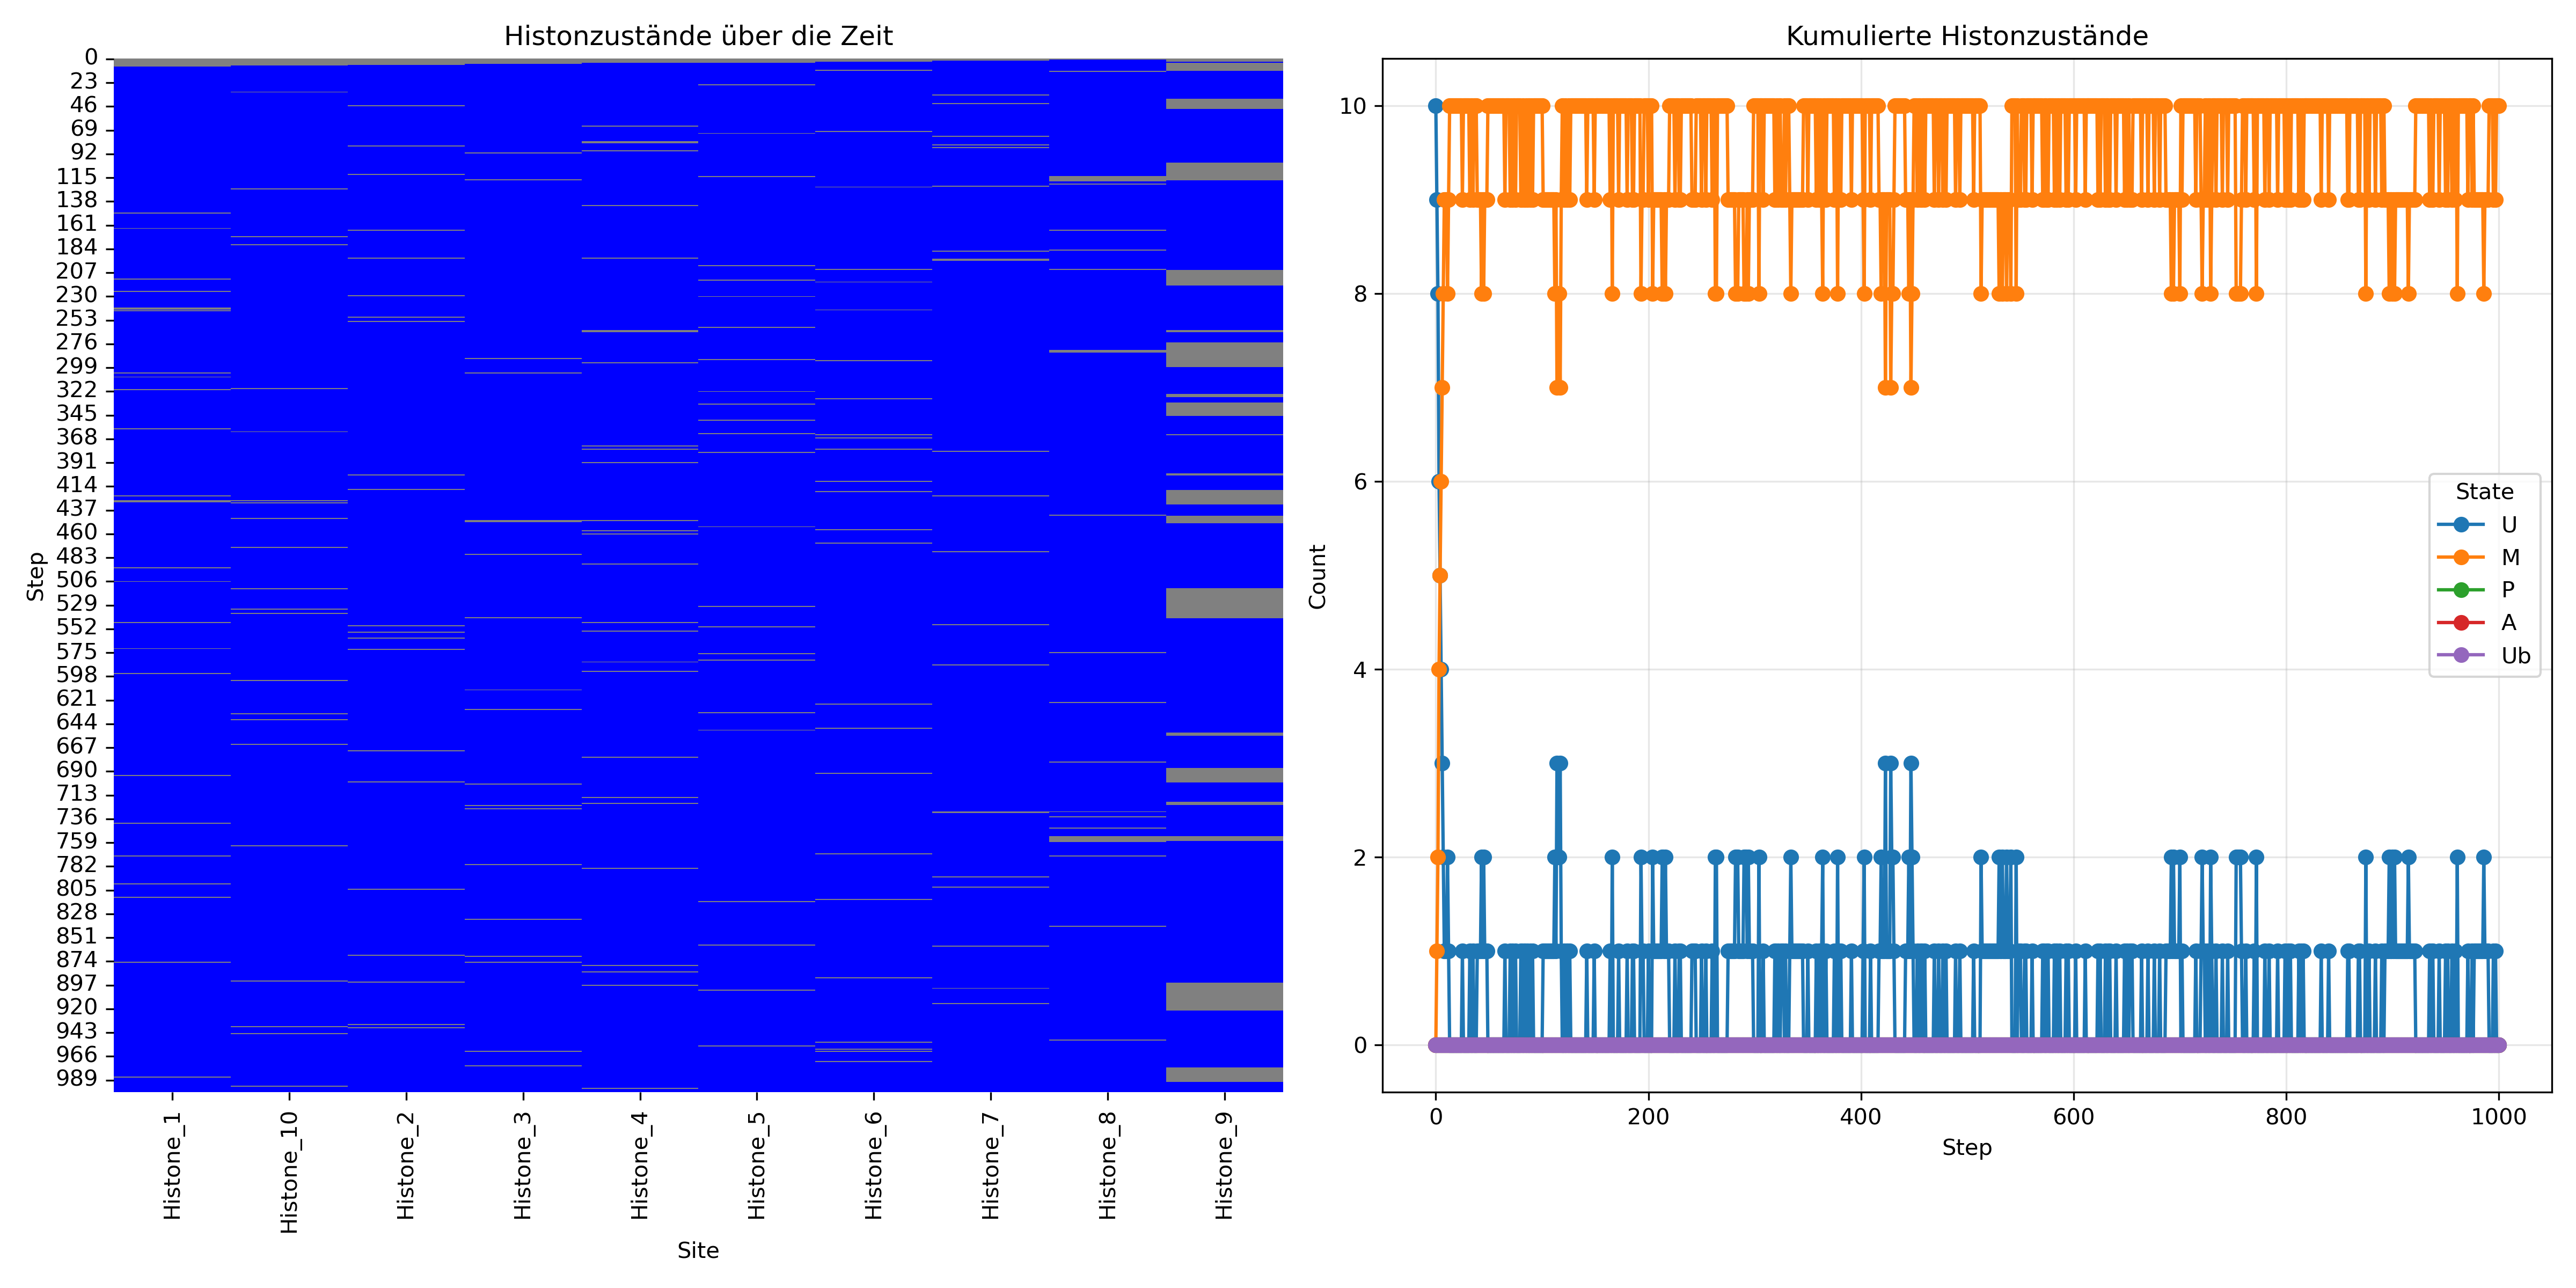
\includegraphics[width=0.9\textwidth]{images/Histone_Fu_1000.png}
  \caption{Visualisierung des stochastischen Modells mit den Wahrscheinlichkeiten für de-novo-methylierung im Tochterstrang und Fehlerrate der Methylierungserhaltung aus Fu et al. (2010) und 1000 Iterationen. \cite{fu-2010}}
  \label{fig:Fu_1000}
\end{figure}

\begin{figure}[htbp]
  \centering
  
\includegraphics[width=0.9\textwidth]{images/Fu_eq.png}
  \caption{Equilibrium bei Fu et al.}
  \label{fig:Fu_eq}
  \end{figure}

\begin{figure}[htbp]
\centering
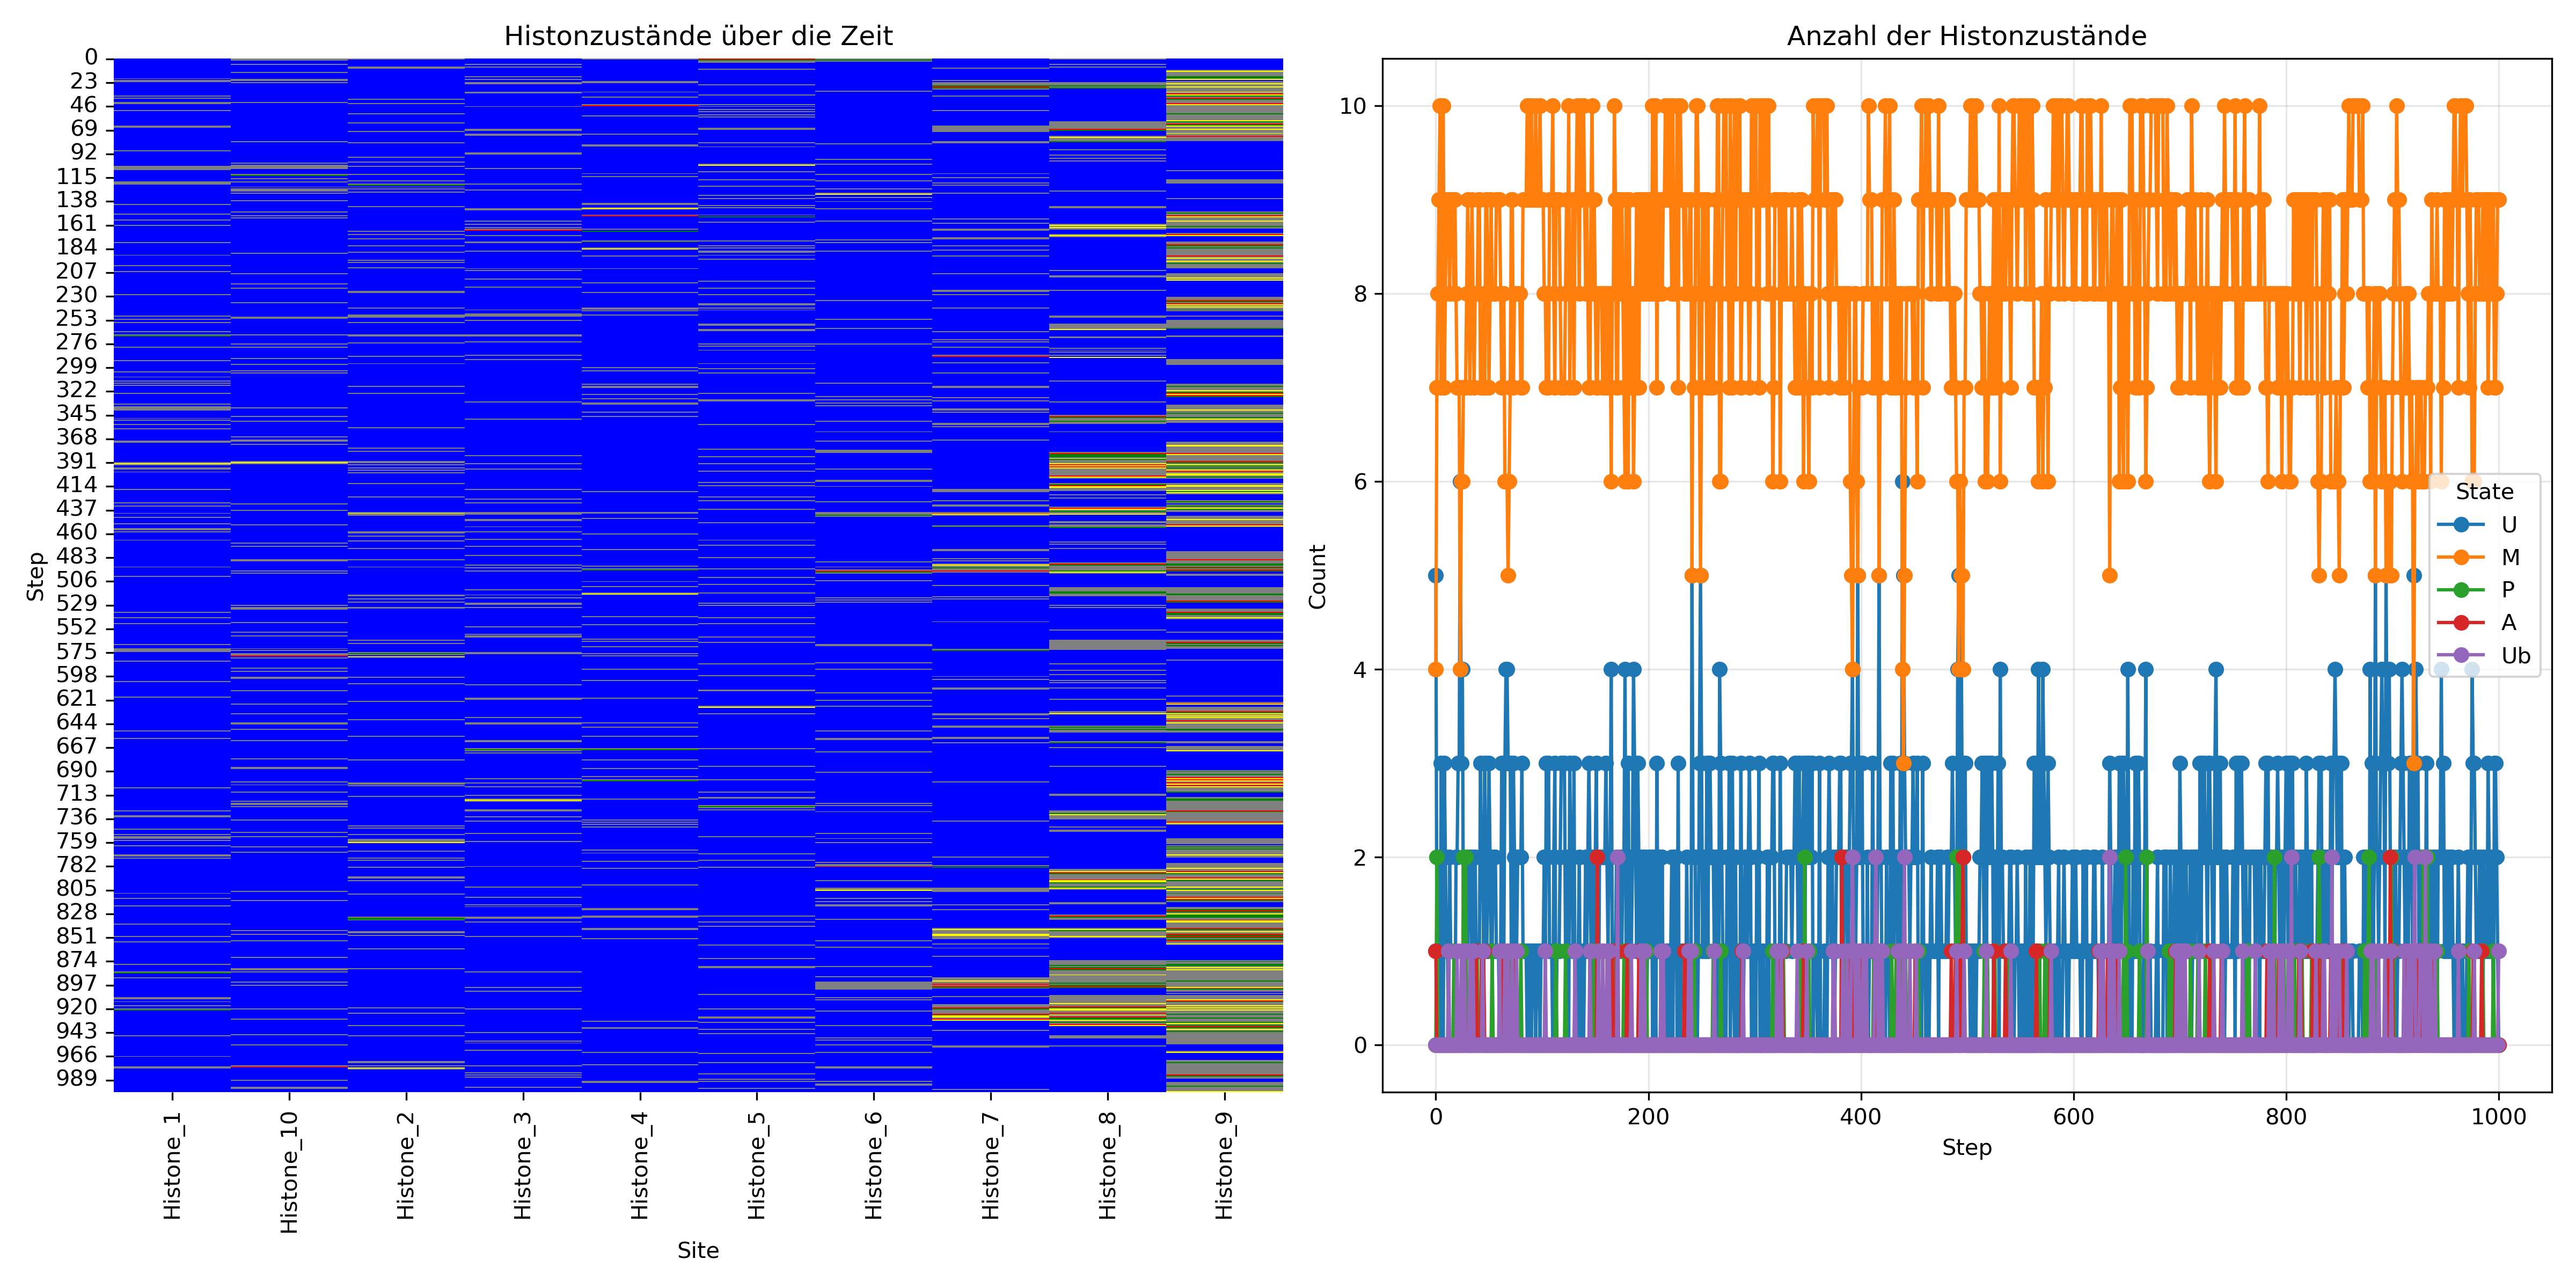
\includegraphics[width=0.9\textwidth]{images/Histone_Prohaska_1000.png}
\caption{Visualisierung des deterministischen Modells: links Heatmap der Zustände über die Zeit, rechts Häufigkeiten der Zustände.}
\label{fig:P_1000}
\end{figure}

\begin{figure}[htbp]
\centering
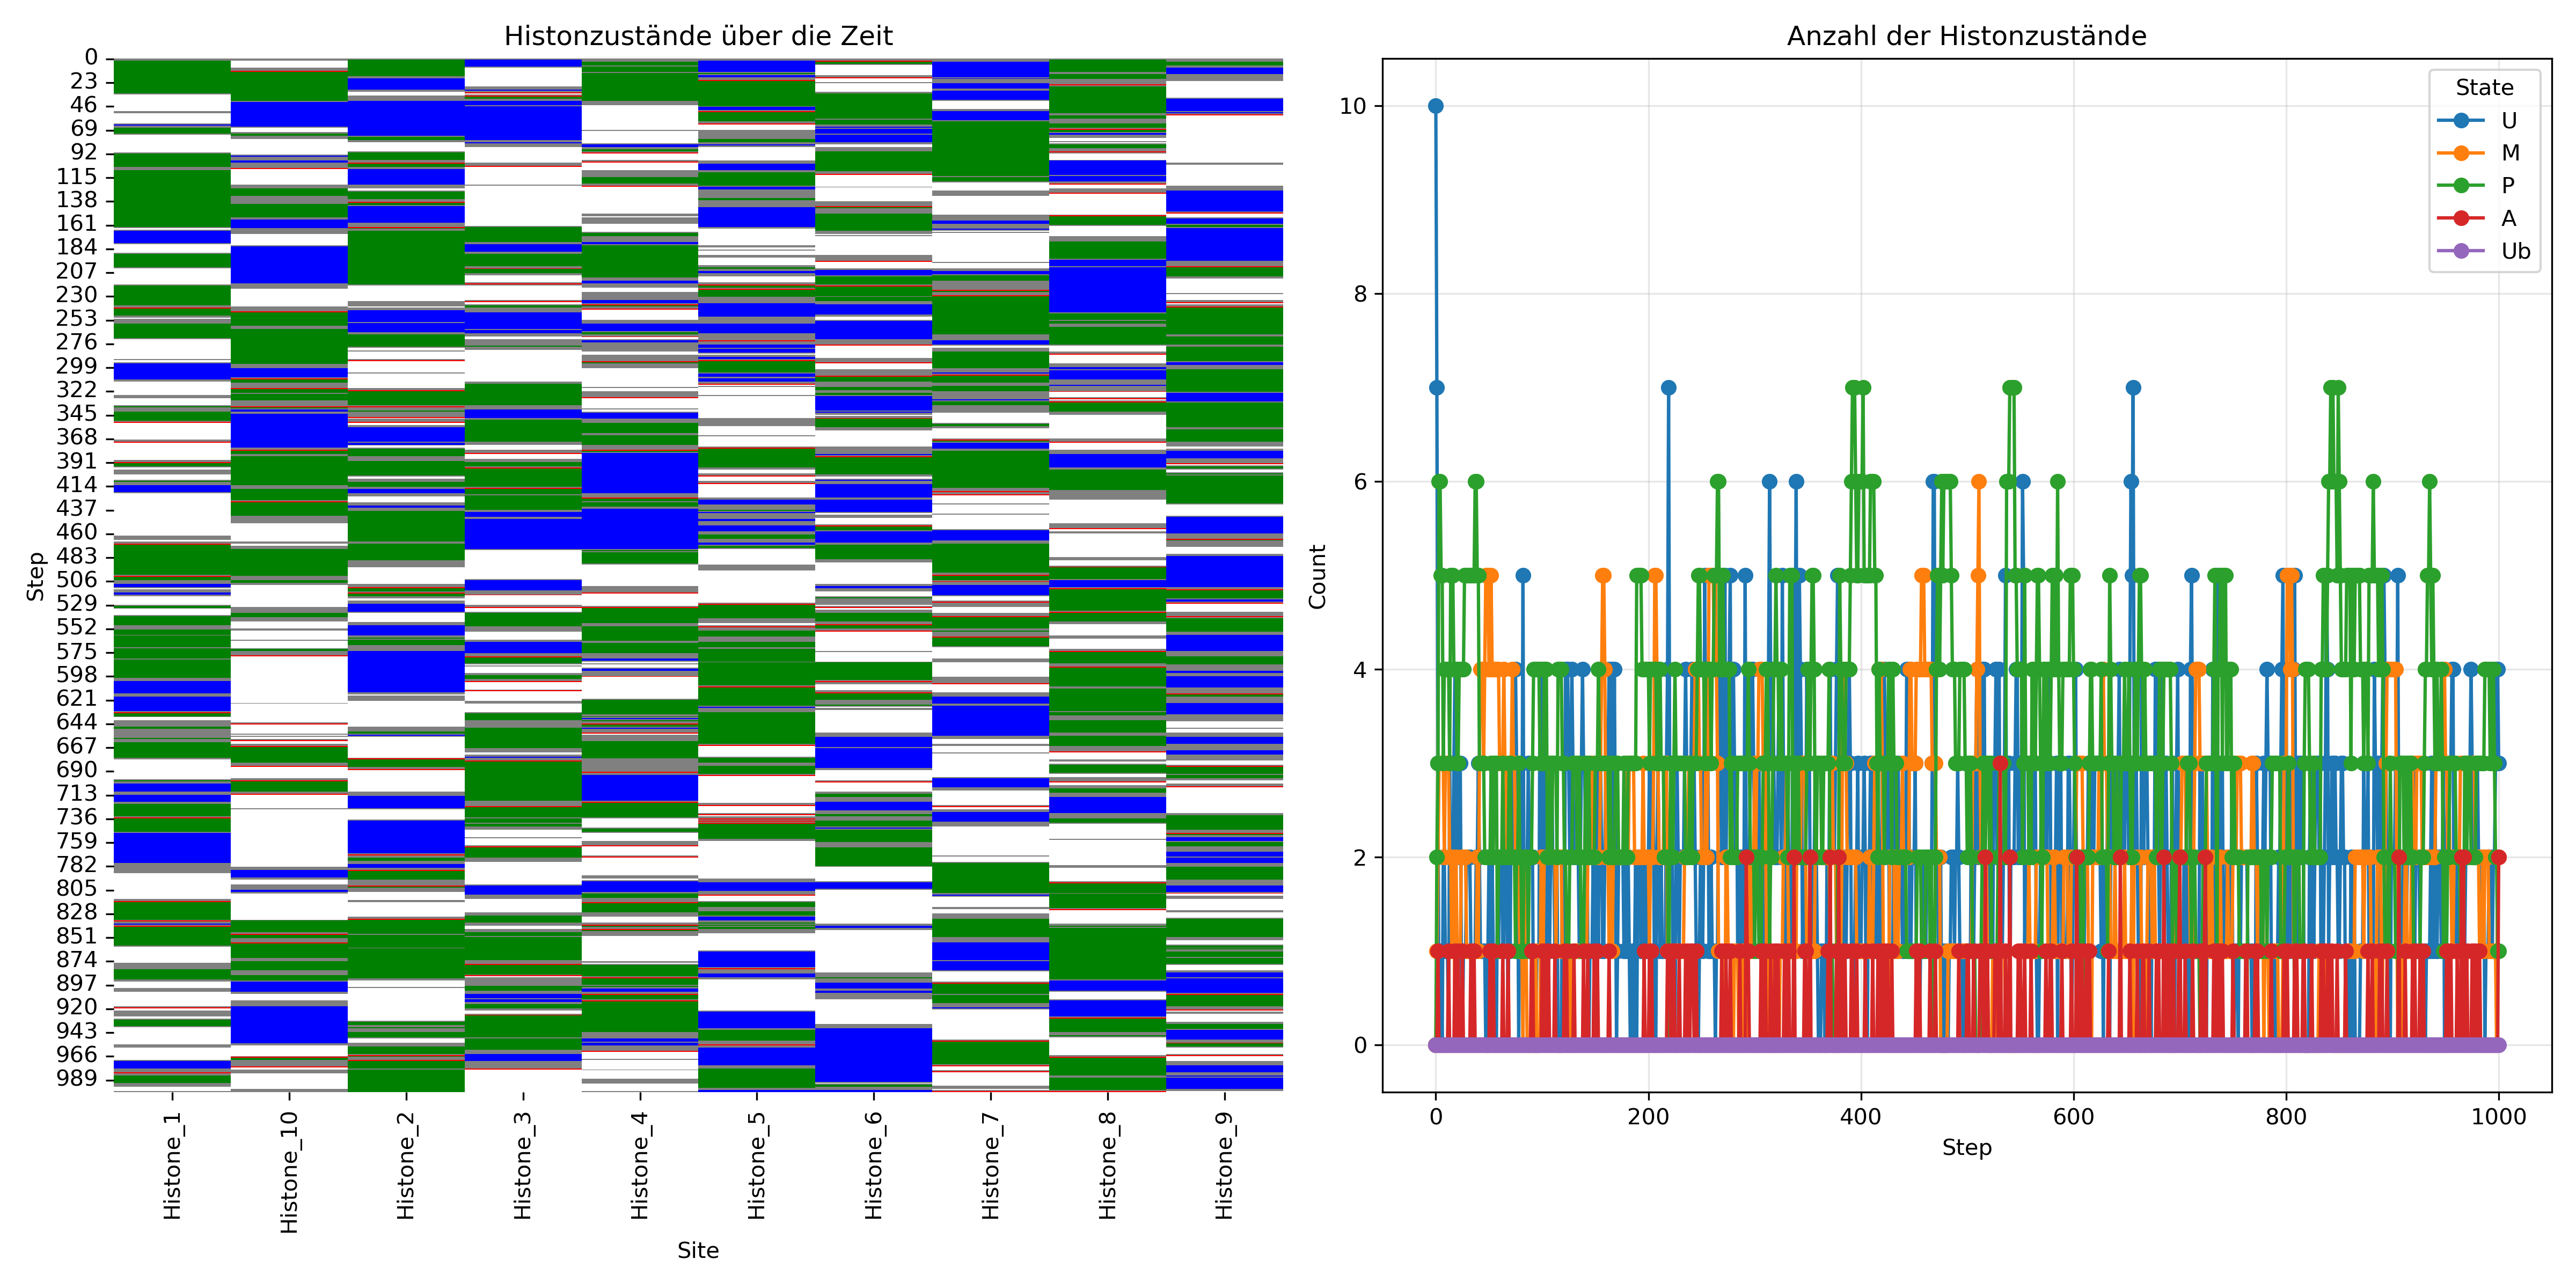
\includegraphics[width=0.9\textwidth]{images/Histone_Markov_1000.png}
\caption{Visualisierung des stochastischen Modells: links Heatmap der Zustände über die Zeit, rechts Häufigkeiten der Zustände.}
\label{fig:M_1000}
\end{figure}

\begin{figure}[htbp]
  \centering
  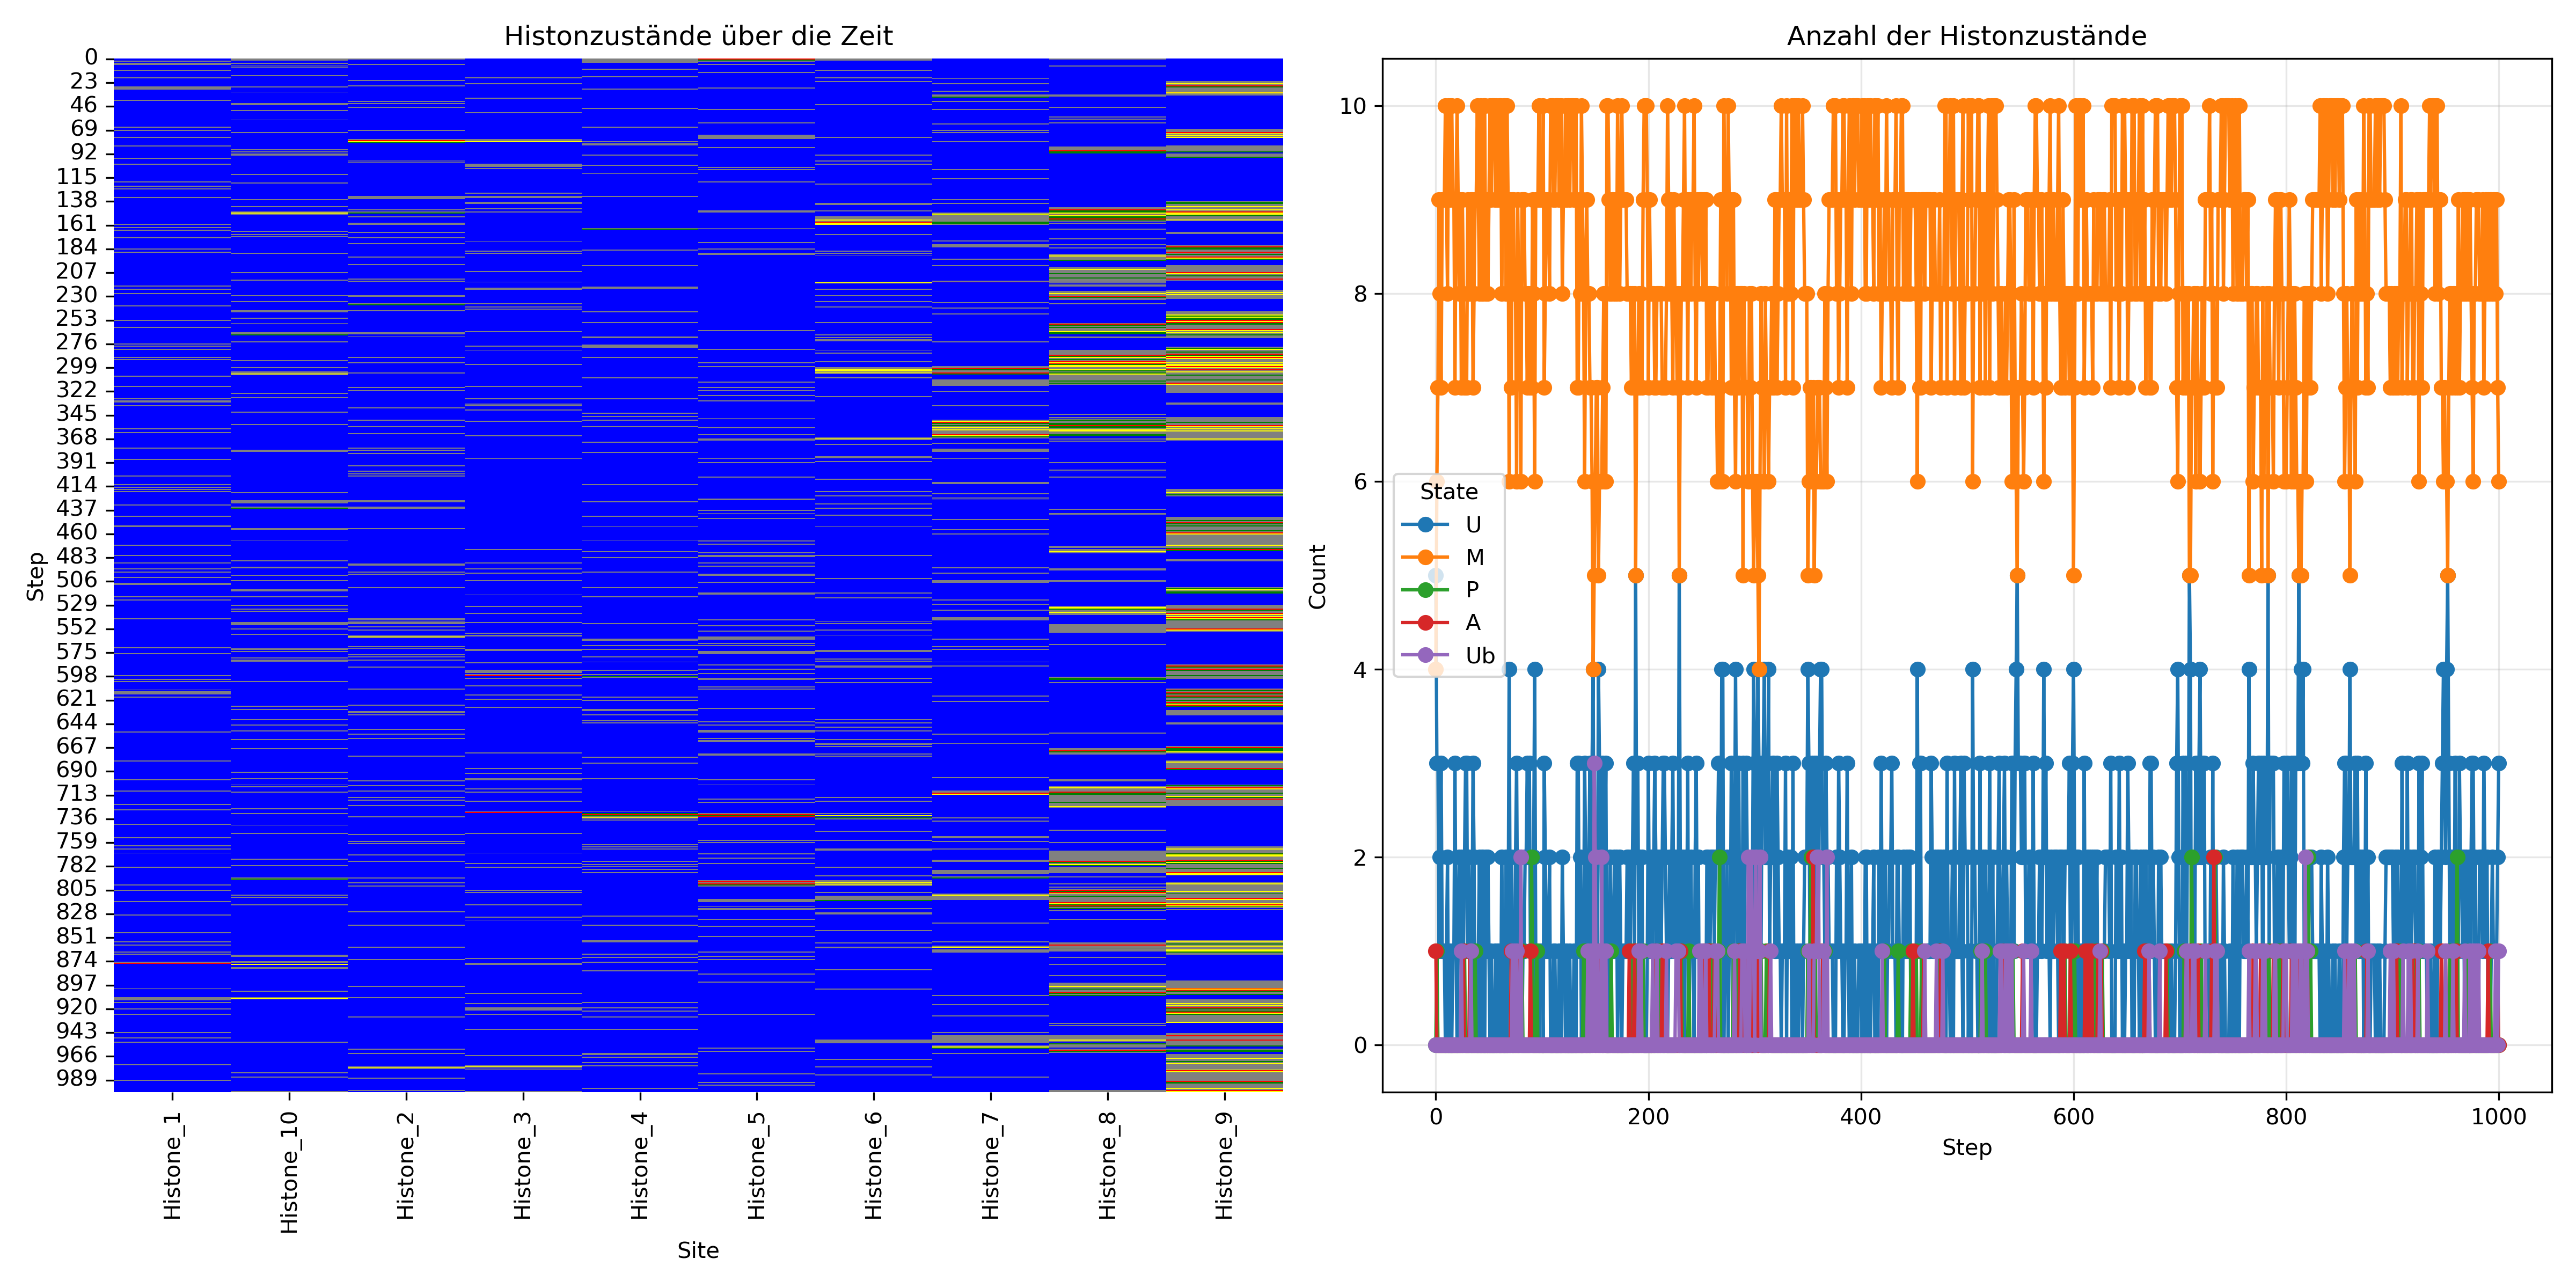
\includegraphics[width=0.9\textwidth]{images/Histone_Prohaska_and_Markov_1000.png}
  \caption{Visualisierung des gemischten Modells: links Heatmap der Zustände über die Zeit, rechts Häufigkeiten der Zustände.}
  \label{fig:PM_1000}
\end{figure}

\begin{figure} [htbp]
  \centering
  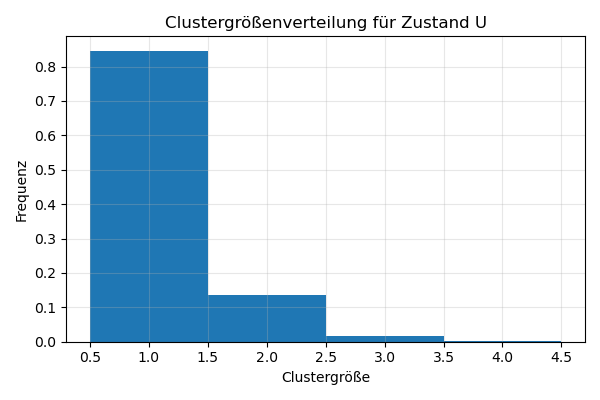
\includegraphics[width=0.9\textwidth]{images/Histone_Prohaska_and_Markov_1000_cluster.png}
  \caption{Clustergröße von Unmethylierten Zuständen im Prohaska und Markov Modell}
  \label{fig:PM_1000_C}
  \end{figure}

\begin{figure}
  \centering
  
\includegraphics[width=0.9\textwidth]{images/Histone_Prohaska_and_Markov_1000_autocor.png}
  \caption{Autokorrelation im deterministischen Modell}
  \label{fig:PM_1000_A}
\end{figure}


\begin{footnotesize}
\newpage
\bibliographystyle{unsrt}
\bibliography{own.bib}
\end{footnotesize}

\end{document}
